% !TEX root = ../phd-thesis.tex

\chapter{Local Completeness Logic}\label{ch:lcla}
\todo[inline]{TODO list}
\begin{itemize}
	\item Change the intro to introduce the "research question"
	\item Less "spoilers" of the results (they will be in the conclusions of the chapter)
\end{itemize}

In this chapter, we extend $\LCLA$ with new capabilities. We investigate the possibility of relaxing point (3) of Theorem~\ref{th:sota:lcl-soundness} to $\denot{\regr}^{A} \alpha(P) = \alpha(Q)$ to achieve extensional soundness, i.e., to untie the set of properties that can be proved about the function computed by the program from the way the program is written . To do so, we follow the idea introduced in~\cite{BGGR23} of \emph{changing the abstract domain} during the analysis, possibly in different ways for different portions of the code.
While~\cite{BGGR23} proposes a single rule for domain refinement, we study here both \emph{refinement} and \emph{simplification} rules for $\LCLA$.
Moreover, we study here how to weaken the hypothesis of Galois connection: the whole theory of completeness is based on the existence of a best approximation for concrete points, but this is not always available in practical instances~\cite{CC92}.

The content of this chapter is based on~\cite{ABG23}.

\section{Motivation}

While any $\LCLA$ valid triple allows to prove both correctness and incorrectness, a very powerful capability, proving an $\LCLA$ triple can be challenging.
The strongest of the three properties required by $\LCLA$ is point~(3) in Theorem~\ref{th:sota:lcl-soundness}, which is a key property to guarantee that point~(2) holds.
The issue is that requiring the abstract interpreter $\denot{\regc}^{\sharp}_{A}$ to be locally complete is an \emph{intensional} property, because the evaluation of $\denot{\regc}^{\sharp}_{A}$ depends on how the code $\regc$ is written.
In fact, it is well known that the abstract analyses $\denot{\regc_1}^{\sharp}_{A}$ and $\denot{\regc_2}^{\sharp}_{A}$ of two programs $\regc_1$ and $\regc_2$ that compute the same function (i.e., $\denot{\regc_1}=\denot{\regc_2}$) can yield different results.

A weaker requirement that suffices to guarantee the validity of point~(2) is the local completeness of the bca $\denot{\regc}^{A}$ of the function $\denot{\regc}$, which is an \emph{extensional} property: it only depends on the abstract domain $A$ and on the computed function $\denot{\regc}$ associated with $\regc$, not on the way $\regc$ is composed. In its original formulation, $\LCLA$ exploits $\denot{\regc}^{\sharp}_{A}$ instead of $\denot{\regc}^{A}$ because the second can be as hard to compute as the concrete semantics $\denot{\regc}$ and because the sequential composition of bcas is not necessarily a bca itself.

The difference between $\denot{\regc}^{A}$ and $\denot{\regc}^{\sharp}_{A}$ is exemplified below:
\begin{example}[Extensional and intensional properties]\label{ex:intro-ext-vs-int}
	Consider the concrete domain $\pow(\setZ)$ of sets of integers and the abstract domain of signs given below:
	\begin{center}
%		\begin{tikzpicture}[scale=0.7,shorten >=-2pt, shorten <=-2pt]
%			\draw (-1,0) node[name=1] {\footnotesize$\varnothing$};
%			\draw (-2,1) node[name=2] {\footnotesize$\setZ_{<0}$};
%			\draw (-1,1) node[name=3] {\footnotesize$\setZ_{=0}$};
%			\draw (0,1) node[name=4] {\footnotesize$\setZ_{>0}$};
%			\draw (-2,2) node[name=5] {\footnotesize$\setZ_{\leq 0}$};
%			\draw (-1,2) node[name=8] {\footnotesize$\setZ_{\neq 0}$};
%			\draw (-0,2) node[name=6] {\footnotesize$\setZ_{\geq 0}$};
%			\draw (-1,3) node[name=7] {\footnotesize$\setZ$};
%			\draw (-3.5,2.9) node[name=n] {{\normalsize $\Sign$}};
%			
%			
%			\draw[semithick] (1) -- (2);
%			\draw[semithick] (1) -- (3);
%			\draw[semithick] (1) -- (4);
%			\draw[semithick] (2) -- (5);
%			\draw[semithick] (2) -- (8);
%			\draw[semithick] (3) -- (5);
%			\draw[semithick] (3) -- (6);
%			\draw[semithick] (4) -- (6);
%			\draw[semithick] (4) -- (8);
%			\draw[semithick] (5) -- (7);
%			\draw[semithick] (6) -- (7);
%			\draw[semithick] (8) -- (7);
%		\end{tikzpicture}
		\includegraphics{sign-domain.pdf}
	\end{center}
	The meaning of each abstract elements of $\Sign$ is to represent concrete values that satisfy the respective property: for instance, $\gamma(\setZ_{< 0}) = \{ n \in \setZ \svert n < 0 \}$ and $\alpha( \{ 0; 1; 100 \}) = \setZ_{\ge 0}$.
	The bca of a concrete function $f: \pow(\setZ) \to \pow(\setZ)$ is defined as $f^{\Sign}\eqdef \alpha~f~\gamma: \Sign \to \Sign$.
	
	Consider the simple program fragment 
	$$\regc \eqdef \code{x := x + 1; x := x - 1}\ .$$
	
	Its denotational semantics $\denot{\regc}$ is the identity function $\id_{\setZ}$, so its bca $$\denot{\regc}^{\Sign} \eqdef \alpha~\id_{\setZ}~\gamma = \id_{\Sign}$$
	is just the abstract identity. We say that $\denot{\regc}^{\Sign}$ is \emph{extensional} because it only depends on the function computed by $\regc$, i.e., its denotational semantics. However, an analyser does not know the semantics of $\regc$, so it has to analyse the program syntactically, breaking it down in elementary pieces and gluing the results together. So for instance, starting from the concrete point $P = \{ 1 \}$ the analysis first abstracts it to the property $\alpha(P) = \setZ_{> 0}$, then it computes
	\begin{align*}
		\denot{\regc}^{\sharp}_{\Sign} (\setZ_{> 0}) &= \denot{\code{x := x - 1}}^{\sharp}_{\Sign} \denot{\code{x := x + 1}}^{\sharp}_{\Sign} (\setZ_{> 0}) \\
		&= \denot{\code{x := x - 1}}^{\sharp}_{\Sign} (\setZ_{> 0}) = \setZ_{\ge 0} .
	\end{align*}
	Analogous calculations for all properties in $\Sign$ yields the abstraction
	\[
	\denot{\regc}^{\sharp}_{\Sign}(a) = \begin{cases*}
		\varnothing & if $a = \varnothing$ \\
		\setZ_{\ge 0} & if $a \in \{ \colorbox{lightgray}{$\setZ_{= 0}$}, \colorbox{lightgray}{$\setZ_{> 0}$}, \setZ_{\ge 0} \}$ \\
		\setZ_{< 0} & if $a = \setZ_{< 0}$ \\
		\setZ & if $a \in \{ \colorbox{lightgray}{$\setZ_{\le 0}$}, \colorbox{lightgray}{$\setZ_{\neq 0}$}, \setZ \}$ 
	\end{cases*}
	\]
	that, albeit sound, is less precise than $\id_{\Sign}$ (we highlight with a gray background all inputs on which $\denot{\regc}^{\sharp}_{\Sign}$ loses accuracy). 
	
	The program $\regc$ is equivalent to the command $\code{skip}$, because $\denot{\code{skip}}=\id_{\setZ}$, and thus $\regc$ and $\code{skip}$ are assigned the same bca $\denot{\code{skip}}^{\Sign} = \denot{\code{skip}}^{\Sign} =  \id_{\Sign}$.
	However, $\denot{\code{skip}}^{\sharp}_{\Sign} = \id_{\Sign} \neq \denot{\regc}^{\sharp}_{\Sign}$, exposing the \emph{intensional} essence of the abstract interpreter: the abstraction depends on how the program is written and not only on its semantics.\footnote{While it falls outside the scope of this thesis, we refer the interested reader to, e.g.,~\cite{BGGGP19,BRZ22} for more about intensional and extensional abstract properties.}
\end{example}

The possibility of weakening point~(3) from being an intensional requirement based on $\denot{\regc}^{\sharp}_A$ to an extensional one based on bcas $\denot{\regc}^A$ has several nice consequences.
First, the local completeness of $\denot{\regc}^A$ is enough to guarantee that points~(1-2) hold.
Second, while the proof system itself provides an intensional analysis, because its rules are defined inductively on the program syntax, the information it produces is more precise, in the sense that the property associated with triples is extensional: no precision is lost because of the approximation introduced by the intensional abstract interpreter.
Third, it allows the proof system to derive more triples than the original one, because bcas can be locally complete also in cases where the abstract interpreter is not (but not vice versa).
Finally, since extensional properties are irrespective of how the program is written, this possibility provides the potential for deriving exactly the same triples for equivalent programs.

Moreover, we study how to circumvent another limitation of $\LCLA$. Since that the whole theory of completeness in abstract interpretation is based on the framework of Galois connection, $\LCLA$ cannot be applied to some known instances of abstract domains widely used in static analysis, such as convex polyhedra abstractions~\cite{CH78}. To this end, we exploit abstract convexity to relax the hypothesis of existence of an abstraction function $\alpha$.

\paragraph{Locally complete refinements.}
Abstract domains are ordered by refinement. 
Intuitively, a domain refines another if it has more abstract elements and thus is more concrete.
In general, an analysis in a more concrete domain is more precise. 
However, $\LCLA$ requires local completeness and it is known that the standard notion of (global) completeness is not necessarily preserved by domain refinement~\cite{GRS00}. 
For instance, a common way to combine two different abstract domains is their reduced product~\cite{cousot79}, but it is not always the case that the analysis in the reduced product is (locally) complete, even when it is such in the two domains separately. 

We present three rules for domain refinement in $\LCLA$ and compare their expressiveness and usability. All of them provide extensional guarantees, in the sense that point~(3) is replaced by the property:
\emph{the abstract domain $A$ is locally complete for the (extensional) bca $\denot{\regc}^{A}$ on input $P$.}

The first one is called \lclrule{refine\mbox{-}ext}. $\LCLA$ extended with \lclrule{refine\mbox{-}ext} turns out to be \emph{logically complete}: any triple satisfying the above conditions~(1--3) can be proved in our proof system. This is a theoretical improvement with respect to $\LCLA$, that instead was intrinsically incomplete as a logic, i.e., for any non-trivial abstraction $A$ there exists a sound triple that cannot be derived.

While \lclrule{refine\mbox{-}ext} is theoretically interesting, one of its hypothesis is undecidable. Therefore, we propose two more derived rules, \lclrule{refine\mbox{-}int} and \lclrule{refine\mbox{-}pre}, whose premises can be checked effectively and imply the hypotheses of the more general \lclrule{refine\mbox{-}ext}. Surprisingly, it turns out that \lclrule{refine\mbox{-}int} enjoys a logical completeness result too, while \lclrule{refine\mbox{-}pre} is strictly weaker (in terms of strength of the logic, see Example~\ref{ex:refine-pre-incomplete}). While the former can be used in more situations and is at times the best choice, the latter is much simpler and preferable to use in practice whenever possible (see Example~\ref{ex:refine-pre-usefulness}).

\paragraph{Locally complete simplifications.}
% SIMPLIFY
Despite refinement seems the best way to gain precision in the analysis, completeness can also be achieved simplifying the domain~\cite{GRS00}. 
This direction has not been explored yet for $\LCLA$ and we present here a single new rule \lclrule{simplify} for domain simplification. We motivate the reason why a unique simplification rule can be designed and study its property. It turns out that simplification is strictly weaker than refinement: \lclrule{simplify} only prove local completeness of the intensional abstraction $\denot{\regc}^{\sharp}_{A}$ on input $P$ and is bound by intrinsic incompleteness (Theorem~\ref{th:intrinsic-incompl-simplify}). However, it enjoys some interesting practical applications.

\paragraph{Expressiveness.}

\begin{figure}[t]
	\centering
	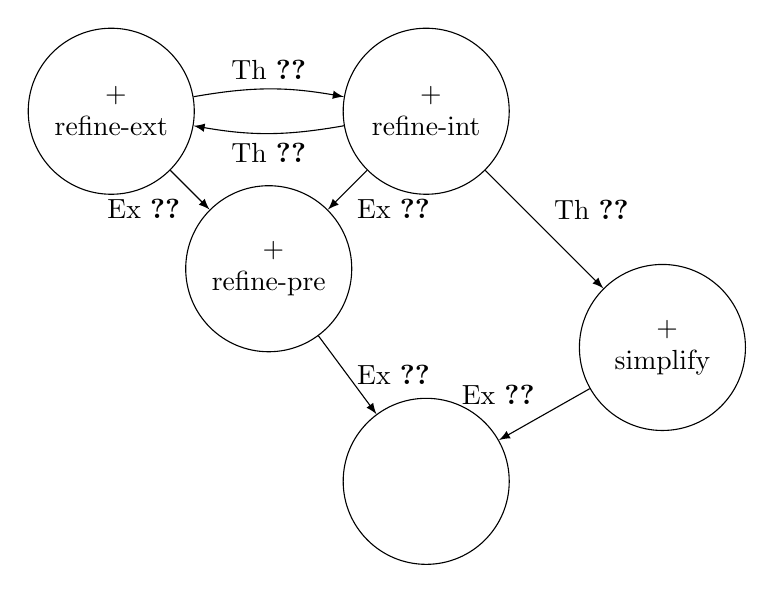
\begin{tikzpicture}
		\node[draw,circle,minimum size=6em] (LCL) at (0, -0.2) {$\LCLA$};
		\node[draw,circle,minimum size=6em,align=center] (RefPre) at (-2, 2.5) {$\LCLA$ + \\ \lclrule{refine\mbox{-}pre}};
		\node[draw,circle,minimum size=6em,align=center] (RefInt) at (0,4.5) {$\LCLA$ + \\ \lclrule{refine\mbox{-}int}};
		\node[draw,circle,minimum size=6em,align=center] (RefExt) at (-4,4.5) {$\LCLA$ + \\ \lclrule{refine\mbox{-}ext}};
		\node[draw,circle,minimum size=6em,align=center] (Simpl) at (3,1.5) {$\LCLA$ + \\ \lclrule{simplify}};
		
		\draw[-latex] (RefPre) edge [right] node {Ex~\ref{ex:refine-pre-usefulness}} (LCL);
		\draw[-latex] (Simpl) edge [above left] node {Ex~\ref{ex:simplify-stronger}} (LCL);
		\draw[-latex] (RefExt) edge [below left] node {Ex~\ref{ex:refine-pre-incomplete}} (RefPre);
		\draw[-latex] (RefExt) edge [bend left=10,above] node {Th~\ref{th:refinement-rule-completeness}} (RefInt);
		\draw[-latex] (RefInt) edge [bend left=10,below] node {Th~\ref{th:refine-int-completeness}} (RefExt);
		\draw[-latex] (RefInt) edge [below right] node {Ex~\ref{ex:refine-pre-incomplete}} (RefPre);
		\draw[-latex] (RefInt) edge [above right] node {Th~\ref{th:refine-int-completeness}} (Simpl);
	\end{tikzpicture}
	\caption{Relations between the new proof systems}\label{fig:rules-comparison-graph}
\end{figure}

We present a pictorial comparison among the expressiveness of the various proof systems in Fig.~\ref{fig:rules-comparison-graph}. The bottom node of the diagram represents the original proof system $\LCLA$ (see Fig.~\ref{fig:lcla-rules}). Each other node represents the original proof system $\LCLA$ (see Fig.~\ref{fig:sota:lcla-rules}) extended with the single rule mentioned in the balloon. Each arrow corresponds to an expressivity result: all triples provable in the target system are also provable in the source system, which is thus more powerful. The labels of the arrows point out the result that justifies the claim. The two mutual arrows between the two topmost nodes indicate that the two proof systems are logically equivalent, i.e., they can prove the same triples. For presentation purposes, we omit arrows obtained by transitivity.
%On the other hand, $\LCLA$ extended with only \lrule{refine\mbox{-}pre} is strictly weaker than \lrule{refine\mbox{-}ext} and \lrule{refine\mbox{-}int} and strictly stronger than plain $\LCLA$.

\section{Locally Complete Refinement}

\section{Locally Complete Simplification}

\section{Exploiting Convexity}

\section{Conclusions}
